\documentclass[11pt]{article}
\usepackage[utf8]{inputenc}
\usepackage[margin=0.8in]{geometry}
\usepackage{amsfonts, amsmath}
\usepackage{tikz}
\usepackage[nobreak=false]{mdframed}
\usepackage{pgf}
\usepackage{mathtools}
\usepackage{bbm}
\usepackage{graphicx}
\usepackage{url}
\usepackage{enumerate}
\usepackage{amsthm,amssymb}
\usepackage{minted}
\setlength\parindent{0pt}
\newcommand{\solution}{\subsection*{Solution:}}
\newcommand{\Lagr}{\mathcal{L}}

\begin{document}

\title{EE 240C Homework 2}
\author{Vighnesh Iyer}
\date{\today}
\maketitle

\subsection*{Problem 1: Spectral Analysis}
\begin{enumerate}[a)]
    \item Plot the spectrum from 0 to $f_s/2$ using FFT without averaging. The y-axis should be in dBFS while the x axis should be in MHz.

      \begin{center}
        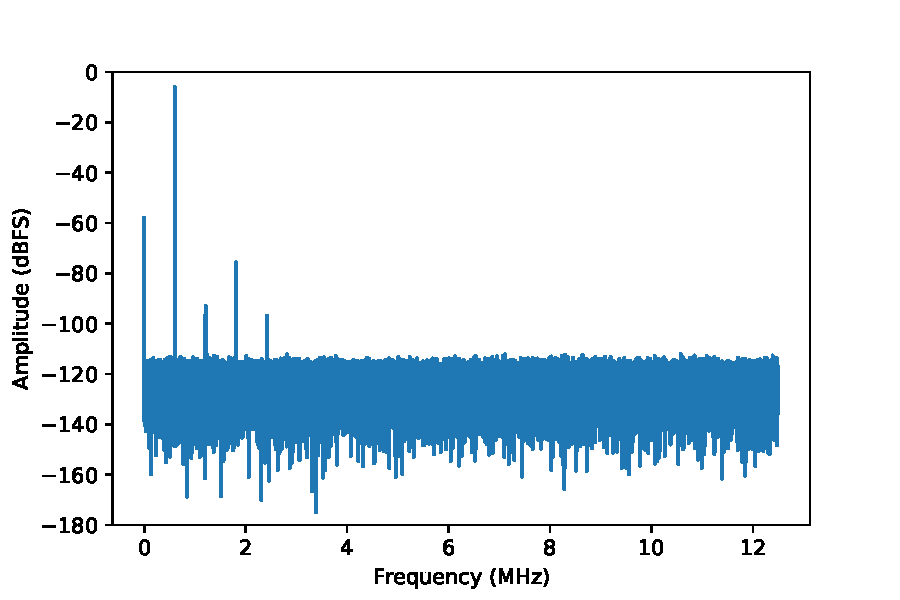
\includegraphics[width=0.6\textwidth]{figs/problem1a.pdf}
      \end{center}

    \item What is the frequency $f_{in}$ of the sinusoidal signal at the input of the ADC?

      The frequency bin with the maximum amplitude is 3171 which corresponds to a frequency of 0.605 MHz.

    \item Compute the following metrics: SNR, SNDR, ENOB, THD, SFDR.

      \begin{itemize}
        \item SNR = $\frac{P_{sig}}{P_{noise}}$ where $P_{noise}$ excludes DC, the signal, and the 2-7th harmonic.

        SNR = $67.9 \text{ dB}$.

        \item SNDR = $\frac{P_{sig}}{P_{noise}}$ where $P_{noise}$ excludes DC and the signal, but includes the harmonics.

          SNDR = $65.65 \text{ dB}$. This is close to the SNR which makes sense since the harmonics are well below the signal.

        \item ENOB = $\frac{SNDR(dB) - 1.76 dB}{6.02 dB}$ = 10.6 bits

        \item THD = $\frac{P_{distortion}}{P_{sig}}$ = -69.5 dB

        \item SFDR = $\frac{P_{spur,max}}{P_{sig}}$ = 69.6 dB
      \end{itemize}

    \item Which non-ideality is limiting the SFDR in this case?

      The INL seems to limiting the SFDR. From the equation in lecture $SFDR = 20 \log_{10}(2^B / INL)$ which for a 12-bit ADC and 1 LSB of INL equals 72 dB SFDR, which is close to the computed value.
\end{enumerate}

\subsection*{Problem 2: Current Steering DACs}

\begin{enumerate}[a)]
  \item To meet the yield requirements for INL and DNL, 2 inequalities can be written. We use 2.6 stddevs as the point for 99\% yield.
\begin{align*}
  \sigma_{INL} &= \frac{1}{2} \sigma_u \sqrt{2^B} = \frac{1}{2} \frac{k_u}{\sqrt{A_{unit}}} \sqrt{2^B} \\
  2.6 \sigma{INL} &< 2 \text{ LSB} \\
  A_{unit} &> \left( \frac{2.6}{2} \frac{k_u \sqrt{2^B}}{2} \right)^2
\end{align*}

\begin{align*}
  \sigma_{DNL} &= \sigma_u \sqrt{2^{B_b + 1} - 1} = \frac{k_u}{\sqrt{A_{unit}}} \sqrt{2^{B_b + 1} - 1}\\
  2.6 \sigma{DNL} &< 0.5 \text{ LSB} \\
  A_{unit} &> \left( \frac{2.6 k_u \sqrt{2^{B_b + 1} - 1}}{0.5} \right)^2
\end{align*}

The greater value of $A_{unit}$ from these inequalities will be used to compute the total area.
Values of $B_b$ are swept in Python:

\begin{minted}{python}
ku = 0.03
inl_a_unit = lambda B: ((2.6/2) * (ku * np.sqrt(2**B)) / 2)**2
dnl_a_unit = lambda Bb: ((2.6/0.5) * ku * np.sqrt(2**(Bb+1) - 1))**2
for Bb in range(12):
    a_unit_1 = inl_a_unit(12)
    a_unit_2 = dnl_a_unit(Bb)
    a_unit = max(a_unit_1, a_unit_2)
    area = (2**(12-Bb))*200 + (2**12)*a_unit
    print(Bb, area, a_unit)
\end{minted}

\begin{minted}{text}
0 825579.536384 1.557504
1 415979.536384 1.557504
2 211179.536384 1.557504
3 108779.536384 1.557504
4 57579.536384 1.557504
5 31979.536384 1.557504
6 25459.392512 3.0906719999999996
7 31818.46528 6.20568
8 54136.61081599999 12.435695999999998
9 103572.90188800002 24.895728000000005
10 204845.48403199998 49.815791999999995
11 408590.64832 99.65592
\end{minted}

The optimal point is at $B_b = 6$ and $B_t = 6$.

\item I used the same script as above to generate data to make the plot.
  \begin{center}
    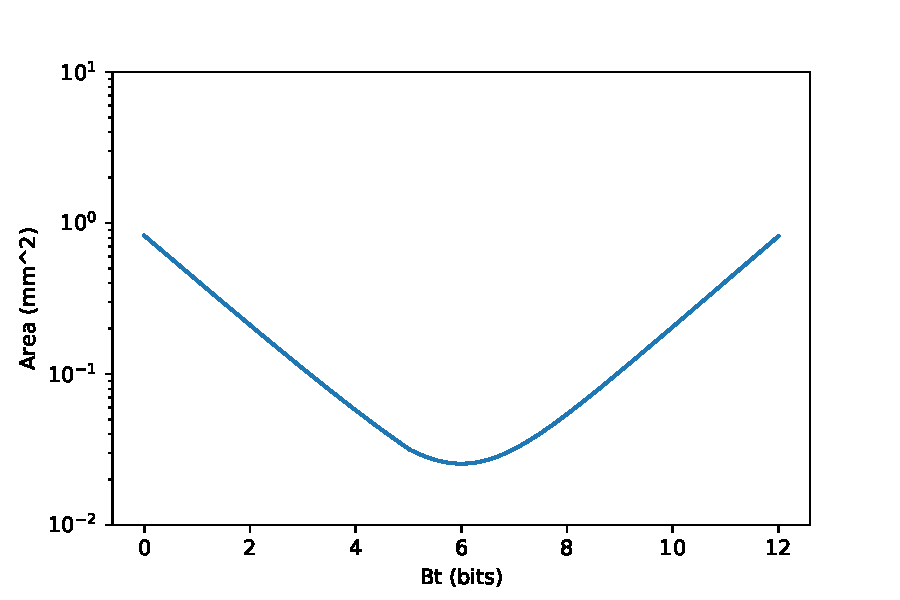
\includegraphics[width=0.6\textwidth]{figs/problem2.pdf}
  \end{center}
\end{enumerate}

\subsection*{Problem 3: Flash ADC}

6-bit flash ADC with ideal resistor string and $V_{ref} = 1.8$V. $\sigma_{offset} = 3$ mV. First and last preamp have no offset.

\begin{enumerate}[a)]
  \item Find $\sigma_{DNL}, \sigma_{INL}$

    From a Maxim document:
    \begin{align*}
      DNL(D) = \left| \frac{V_{D+1} - V_{D}}{V_{lsb,ideal}} - 1 \right|
    \end{align*}
    where $V_{D}$ is the input voltage at which the digital output code transitions to $D$. DNL is defined for $0 < D < 2^N-2$.
    The comparator offset can be added to each term of $V_{D}$:
    \begin{align*}
      DNL(d) &= \left| \frac{(V_{D+1} + V_{off,D+1}) - (V_{D} + V_{off,D})}{V_{lsb,ideal}} - 1 \right| \\
      \sigma_{DNL}^2 &= E[DNL^2] - E[DNL]^2 \\
      E[DNL]^2 &= 0 \\
      E[DNL^2] &\rightarrow \left( \frac{(V_{D+1} + V_{off,D+1}) - (V_{D} + V_{off,D})}{V_{lsb,ideal}} - 1 \right)^2 \\
      &= \left( \frac{V_{lsb} + V_{off,D+1} - V_{off,D} - V_{lsb}}{V_{lsb}} \right)^2 \\
      &= \left( \frac{V_{off,D+1} - V_{off,D}}{V_{lsb}} \right)^2 \\
      &= \frac{V_{off,D+1}^2 - 2 V_{off,D+1} V_{off,D} + V_{off,D}^2}{V_{lsb}^2} \\
      &\rightarrow \frac{E[V_{off,D+1}^2] - 2 E[V_{off,D+1} V_{off,D}] + E[V_{off,D}^2]}{V_{lsb}^2} \\
      &= \frac{2 \sigma_{offset}^2}{V_{lsb}^2} \\
      \sigma_{DNL} &= \sqrt{2} \frac{\sigma_{offset}}{V_{lsb}} = \sqrt{2} \frac{3 \text{ mV}}{1.8 / 2^6} = 0.151 \text{ LSB}
    \end{align*}

    From a Maxim document:
    \begin{align*}
      INL(D) = \left| \frac{V_D - V_{zero}}{V_{lsb}} - D \right|
    \end{align*}
    where $V_{D}$ is the analog value for output code $D$ and $D$ ranges from $0 < D < 2^N - 1$.
    $V_{zero}$ is the minimum analog input for an all zero output code, which in our case is 0 V.

    Adding an offset:
    \begin{align*}
      INL(D) &= \left| \frac{V_{D,nom} + V_{off} - D V_{lsb}}{V_{lsb}} \right| \\
      V_{D,nom} &= V_{lsb} D \\
      INL(D) &= \left| \frac{D V_{lsb} + V_{off} - D V_{lsb}}{V_{lsb}} \right| \\
      &= \left| \frac{V_{off}}{V_{lsb}} \right| \\
      \sigma_{INL} &= \frac{\sigma_{offset}}{V_{lsb}} = 0.11 \text{ LSB}
    \end{align*}

  \item How are $\sigma_{DNL}$ and $\sigma_{INL}$ affected by 4x interpolation $(M = 4)$?

    The effective offset of the preamps is divided by the interpolation factor, so both $\sigma_{INL}$ and $\sigma_{DNL}$ should be reduced by 4x.
\end{enumerate}

\subsection*{Problem 4: kT/C Noise}

\begin{align*}
  C &= 12 kT \left( \frac{2^B}{V_{FS}} \right)^2 \\
  2.2 R C &= \frac{1}{2 f_s} \\
  V_{FS} &= \sqrt{2 f_s \cdot 2.2R \cdot 12 kT \cdot 2^{B^2}} \\
  \overline{V_{n}^2} &= \frac{k T}{C} = \frac{2 f_s \cdot 2.2R \cdot 12 kT}{12}
\end{align*}
\end{document}
